%
% 3-laurentreihen.tex -- Laurent-Reihen
%
% (c) 2025 Prof Dr Andreas Müller
%
\section{Laurent-Reihen und meromorphe Funktionen
\label{buch:analytisch:section:laurentreihen}}
\kopfrechts{Laurent-Reihen}
Analytische Funktionen sind immer auf einem Kreisgebiet um den
Entwicklungspunkt definiert.
Der Radius dieses Gebietes wird beschränkt durch die nächstliegende
Singularität der Funktion.
So ein Kreisgebiet ist einfach zusammenhängend, jeder geschlossene
Weg lässt sich in einen Punkt zusammenziehen.
Der nächstschwierigere aber auch etwas interessantere Fall ist,
dass eine holomorphe Funktion nur in einem Ringgebiet definiert ist.
Die einfachsten Beispiele dafür sind die Funktion $z^{-n}$ mit
$n\in\mathbb{N}\setminus\{0\}$, die auf $\mathbb{C}\setminus\{0\}$
definiert sind.
In diesem Abschnitt werden Funktionen auf einem Ringebiet genauer
untersucht und es wird eine Erweiterung der Potenzreihenentwicklung
für negative Potenzen, die Laurent-Reihe, konstruiert.

%
% 31-ring.tex -- Funktionen auf einem Ringgebiet
%
% (c) 2026 Prof Dr Andreas Müller
%
\subsection{Funktionen auf einem Ringgebiet}
%
% fig-ring.tex
%
% (c) 2026 Prof Dr Andreas Müller
%
\begin{figure}
\centering
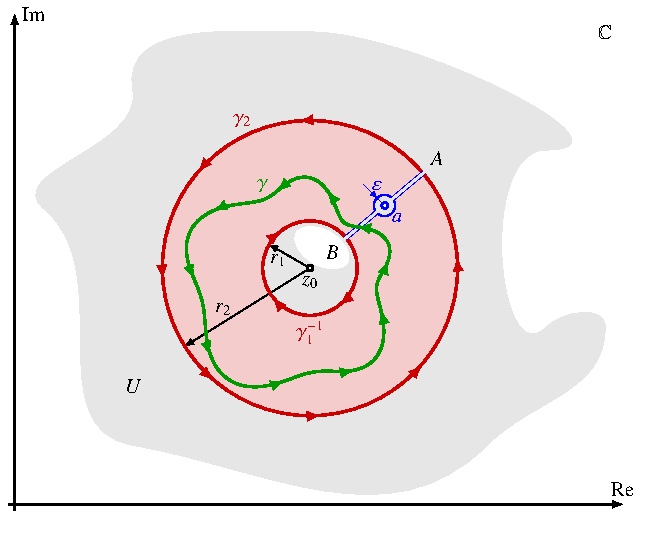
\includegraphics{chapters/040-analytisch/images/ring.pdf}
\caption{Die Funktion $f\colon U\to\mathbb{C}$ kann mithilfe eines
Pfadintegrals über den roten Rand berechnet werden, wodurch sich
die Entwicklung der Funktion in eine Laurent-Reihe finden lässt.
Die Koeffizienten der Laurent-Reihe können aber auch mit dem 
Weg $\gamma$ berechnet werden, der sich im Ringgebiet zu $\gamma_1$
oder $\gamma_2$ deformieren lässt.
\label{buch:analytisch:laurent:fig:ring}}
\end{figure}
%
Wir betrachten eine holomorphe Funktion $f\colon U\to\mathbb{C}$.
Die offene Menge $U$ sei so gestaltet, dass der \emph{Ring}
\[
R(z_0;r_1,r_2)
=
\{
z\in\mathbb{C}
\mid
r_1 \le |z-z_0| \le r_2
\}
\]
in $U$ enthalten ist.
\index{Ringgebiet}%
Abbildung~\ref{buch:analytisch:laurent:fig:ring} zeigt diese Situation.
Das Innere des Rings, der kleine Kreis mit Radius $r_1$ heisst auch
das \emph{Auge} des Rings.
\index{Auge}%

Da die Funktion $f$ im Inneren des kleinen Kreises mit Radius $r_1$ um
den Punkt $z_0$ nicht überall definiert sein muss, ist der Integralsatz
von Cauchy nicht auf den grossen Kreis anwendbar.
Der folgende Satz zeigt, dass es aber trotzdem möglich ist, den Wert von
$f$ in einem beliebigen Punkt des Ringgebietes mit einem Wegintegral
zu berechnen.

\begin{satz}
Seien $\gamma_2$ und $\gamma_1$ die im Gegenuhrzeigersinn durchlaufenen
Randkreise des Ringgebietes $R(z_0;r_1,r_2)$ mit Radien $r_2$ und $r_1$.
Dann gilt
\begin{equation}
f(a)
=
\frac{1}{2\pi i}
\oint_{\gamma_2}
\frac{f(z)}{z-a}
\,dz
-
\frac{1}{2\pi i}
\oint_{\gamma_1}
\frac{f(z)}{z-a}
\,dz
\label{buch:analytisch:laurent:eqn:zweiintegrale}
\end{equation}
für jeden Punkt $a\in R(z_0;r_1,r_2)$.
\end{satz}

\begin{proof}
Der in Abbildung~\ref{buch:analytisch:laurent:fig:ring} dargestellte
Weg, der vom Punkt $A$ ausgehend zunächst dem äusseren Randkreis
folgt bis wieder zurück zum Punkt $A$, dann radial zum Punkt $a$,
in einem Halbkreis vom Radius $\varepsilon$ um den Punkt $a$ und
dann geradlinig weiter bis zum Punkt $B$, von dort im Uhrzeigersinn
um den inneren Randkreis zurück zum Punkt $B$ und erneut radial zum
Punkt $A$, wieder mit einem kleinen, kreisförmigen Umweg vom Radius
$\varepsilon$ um den Punkt $a$.
Die Funktion ist im Inneren des Weges überall holomorph,
nach dem Integralsatz von Cauchy verschwindet das Integral über
den ganzen Weg.

Die radialen Teile werden zweimal in entgegengesetzter Richtung durchlaufen
und heben sich daher weg.
Somit bleiben nur noch die Integrale über die Teile $\gamma_2$,
$\gamma_1^{-1}$ und $\gamma_\varepsilon$, die zusammen das Integral
über die Kette $\gamma_2+\gamma_1^{-1}+\gamma_{\varepsilon}^{-1}$ mit
dem Wert
\[
0
=
\oint_{\gamma_2 + \gamma_1^{-1} + \gamma_{\varepsilon}^{-1}}
\frac{f(z)}{z-a}\,dz 
=
\oint_{\gamma_2}
\frac{f(z)}{z-a}\,dz 
-
\oint_{\gamma_1}
\frac{f(z)}{z-a}\,dz 
-
\oint_{\gamma_{\varepsilon}}
\frac{f(z)}{z-a}\,dz 
\]
ergeben.

Der kleine Kreis $\gamma_\varepsilon$ um den Punkt $a$ kann mit
$t\mapsto \varepsilon e^{2\pi it}$ parametrisiert werden, um das
Integral zu berechnen.
So wird aus dem Integral
\begin{align*}
0
&=
\oint_{\gamma_2} \frac{f(z)}{z-a}\,dz
-
\oint_{\gamma_1} \frac{f(z)}{z-a}\,dz
-
\int_0^1
\frac{f(a+\varepsilon e^{2\pi it})}{a+\varepsilon e^{2\pi it}-a}
\cdot
\frac{d}{dt}
\varepsilon
e^{2\pi it}
\,dt
\intertext{aufgelöst nach dem Integral über $\gamma_\varepsilon$}
\oint_{\gamma_2} \frac{f(z)}{z-a}\,dz
-
\oint_{\gamma_1} \frac{f(z)}{z-a}\,dz
&=
\int_0^1
\frac{f(a+\varepsilon e^{2\pi it})}{\varepsilon e^{2\pi it}}
\cdot
2\pi i\varepsilon e^{2\pi it}
\,dt
\\
&=
2\pi i
\int_0^1
f(a+\varepsilon e^{2\pi it})
\,dt.
\intertext{Das Integral auf der rechten Seite geht für $\varepsilon\to 0$
gegen $f(a)$, wir erhalten also}
&=
2\pi i f(a).
\intertext{Aufgelöst nach $f(a)$ finden wir}
f(a)
&=
\frac{1}{2\pi i}
\oint_{\gamma_2}
\frac{f(z)}{z-a}
\,dz
-
\frac{1}{2\pi i}
\oint_{\gamma_1}
\frac{f(z)}{z-a}
\,dz.
\end{align*}
Damit ist der Satz bewiesen.
\end{proof}

\begin{beispiel}
Wir betrachten die Funktion $f(z)=1/z$ im Ringgebiet $R(0;r_1,r_2)$ und
rechnen die Integralformel~\eqref{buch:analytisch:laurent:eqn:zweiintegrale}
nach.
Mit der Partialbruchzerlegung
\[
\frac{1}{z(z-a)}
=
\frac{1}{a}
\biggl(
\frac{1}{z}
+
\frac{1}{z-a}
\biggr)
\]
können die Integrale aufgespaltet und mit der Cauchy-Integralformel
berechnet werden als
\begin{align*}
\int_{\gamma_2} \frac{f(z)}{z-a}\,dz
&=
\frac1a
\int_{\gamma_2} {\color{darkred}\frac{1}{z}}+\frac{1}{z-a}\,dz
=
{\color{darkred}
\frac1a
\underbrace{
\int_{\gamma_2} \frac{1}{z}\,dz
}_{\displaystyle=2\pi i}
}
+
\frac1a
\underbrace{
\int_{\gamma_2}\frac{1}{z-a}\,dz
}_{\displaystyle=2\pi i}
%
\intertext{und}
\int_{\gamma_1} \frac{f(z)}{z-a}\,dz
&=
\frac1a
\int_{\gamma_1} {\color{darkred}\frac{1}{z}}+\frac{1}{z-a}\,dz
=
{\color{darkred}
\frac1a
\underbrace{
\int_{\gamma_1} \frac{1}{z}\,dz
}_{\displaystyle=2\pi i}
}
+
\frac1a
\underbrace{
\int_{\gamma_1} \frac{1}{z-a}\,dz.
}_{\displaystyle=0}
\end{align*}
Das letzte Integral verschwindet, weil die Funktion $1/(z-a)$ holomorph
ist im Auge des Ringgebietes.
Die Integralformel~\eqref{buch:analytisch:laurent:eqn:zweiintegrale}
wird jetzt zu
\begin{align*}
\frac{1}{2\pi i}
\int_{\gamma_2} \frac{f(z)}{z-a}\,dz
-
\frac{1}{2\pi i}
\int_{\gamma_1} \frac{f(z)}{z-a}\,dz
&=
{\color{darkred}\frac1a} + \frac1a - {\color{darkred}\frac1a}
=
\frac1a
=
f(a).
\end{align*}
Die Integralformel~\eqref{buch:analytisch:laurent:eqn:zweiintegrale}
berechnet tatsächlich den Funktionswert an der Stelle $a$.

Die roten Integrale sind Beiträge der Polstelle im Zentrum des Ringgebietes.
Da sie in beiden Integralen über $\gamma_2$ und $\gamma_1$ auftreten,
heben Sie sich in der Differenz weg, so dass nur noch der Beitrag
der Polstelle des Integranden bei $a$ übrig bleibt.
\end{beispiel}

%
% 32-laurent.tex -- Die Laurent-Reihe
%
% (c) 2026 Prof Dr Andreas Müller
%
\subsection{Die Laurent-Reihe}
Auf einem Kreisgebiet lässt sich eine holomorphe Funktion immer in eine
Potenzreihe entwickeln.
Auf einem Ringgebiet ist dies nicht mehr möglich.
An die Stelle der Potenzreihe tritt ein sogenannte Laurent-Reihe.

\begin{definition}[Laurent-Reihe]
\label{buch:analytisch:laurent:def:laurentreihe}
Eine \emph{Laurent-Reihe} ist eine Reihe der Form
\index{Laurent-Reihe}%
\begin{equation}
f(a)
=
\sum_{k=0}^\infty a_k(a-z_0)^k
+
\sum_{k=1}^\infty b_k(a-z_0)^{-k}
\label{buch:analytisch:laurent:def:laurent}
\end{equation}
mit $a_k\in\mathbb{C}$, $k\in\mathbb{N}$ und $b_k\in\mathbb{C}$,
$k\in\mathbb{N}\setminus\{0\}$.
\end{definition}

Die erste Reihe in
\eqref{buch:analytisch:laurent:def:laurent}
ist eine gewöhnliche Potenzreihen, deren Konvergenzradius wir mit $r_2$
bezeichnen.
Die zweite Reihe können wir auch als
\begin{equation}
\sum_{k=1}^\infty b_k(a-z_0)^{-k}
=
\sum_{k=1}^\infty b_k\biggl(\frac{1}{a-z_0}\biggr)^{k}
\label{buch:analytisch:laurent:def:laurent2}
\end{equation}
schreiben, also als Potenzreihe in $1/(a-z_0)$.
Der Konvergenzradius $\varrho$ dieser Potenzreihe kann mit der
Cauchy-Hadamard-Formel berechnet werden.
Die Reihe~\eqref{buch:analytisch:laurent:def:laurent2}
konvergiert dann für $|a-z_0| > 1/\varrho = r_1$.
Nach dem Satz von Cauchy-Hadamard ist die Laurent-Reihe ist also 
auf dem Ringgebiet $R(z_0;r_1,r_2)$ mit den Radien
\begin{align*}
\frac{1}{r_1}
&=
\limsup_{n\to\infty}\!\sqrt[n]{|b_n|}
&&\text{und}&
r_2
&=
\limsup_{n\to\infty}\!\sqrt[n]{|a_n|}.
\end{align*}
und $r_1 < r_2$ konvergent.

\begin{satz}[Laurent-Reihe]
\label{buch:analytisch:laurent:satz:laurentreihe}
Ist $f$ eine auf einer Umgebung des Ringgebietes $R(z_0;r_1,r_2)$ definierte
holomorphe Funktion, dann kann sie in eine Laurent-Reihe entwickelt werden.
Ist $\gamma$ ein beliebiger Weg im Ringgebiet, der $z_0$ genau einmal
im Gegenuhrzeigersinn umläuft, dann sind die 
Koeffizienten durch
\begin{align}
a_k
&=
\frac{1}{2\pi i}
\oint_{\gamma} 
\frac{f(z)}{(z-z_0)^{k+1}}
\,dz
&&\text{und}&
b_k
&=
\frac{1}{2\pi i}
\oint_{\gamma} 
f(z)(z-z_0)^{k-1}
\,dz
\label{buch:analytisch:laurent:eqn:laurentkoeffizienten}
\end{align}
gegeben.
\end{satz}

\begin{proof}
Wir berechnen jetzt die beiden Integrale in
\eqref{buch:analytisch:laurent:eqn:zweiintegrale} separat mit
verschiedenen Entwicklungen des Integranden.
Das erste Integral über den äusseren Randkreis $\gamma_2$ des Ringgebietes
lässt sich wie früher in eine geometrische Reihe
\begin{equation}
\frac{1}{2\pi i}
\oint_{\gamma_2}
\frac{f(z)}{z-a}
\,dz
=
\sum_{k=0}^\infty
\biggl(
\underbrace{
\frac{1}{2\pi i}
\oint_{\gamma_2}
\frac{f(z)}{(z-z_0)^{k+1}}
\,dz
}_{\displaystyle =a_k}
\biggr)
(a-z_0)^k
=
\sum_{k=0}^\infty a_k(a-z_0)^k
\label{buch:analytisch:laurent:eqn:integral1}
\end{equation}
entwickeln.

Für das Integral über den inneren Randkreis  $\gamma_1$
verwenden wir die geometrische Reihe
\begin{align*}
\frac{1}{z-a\mathstrut}
&=
\frac{1}{z-z_0-(a-z_0)\mathstrut}
\\
&=
-
\frac{1}{a-z_0}\cdot \frac{1}{1-\displaystyle\frac{z-z_0\mathstrut}{a-z_0}}
=
-
\frac{1}{a-z_0}
\sum_{k=0}^\infty \biggl(\frac{z-z_0}{a-z_0}\biggr)^k
\\
&=
-
\sum_{k=0}^\infty \frac{1}{(a-z_0)^{k+1}}(z-z_0)^k.
\end{align*}
Damit kann das Integral über $\gamma_1$ als
\begin{align}
-
\frac{1}{2\pi i}
\oint_{\gamma_1}
\frac{f(z)}{z-a}
\,dz
&=
\frac{1}{2\pi i}
\oint_{\gamma_1}
\sum_{k=0}^\infty
f(z)(z-z_0)^k
\frac{1}{(a-z_0)^{k+1}}
\,dz
\notag
\\
&=
\sum_{k=0}^\infty
\biggl(
\frac{1}{2\pi i}
\oint_{\gamma_1}
f(z) (z-z_0)^k
\,dz
\biggr)
\cdot
\frac{1}{(a-z_0)^{k+1}}.
\notag
\intertext{geschrieben werden.
Durch Verschiebung des Summationsindex wird daraus}
-
\frac{1}{2\pi i}
\oint_{\gamma_1}
\frac{f(z)}{z-a}
\,dz
&=
\sum_{k=1}^\infty
\biggl(
\underbrace{
\frac{1}{2\pi i}
\oint_{\gamma_1}
f(z) (z-z_0)^{k-1}
\,dz
}_{\displaystyle =b_k}
\biggr)
\cdot
\frac{1}{(a-z_0)^k}
\notag
\\
&=
\sum_{k=1}^\infty
b_k
\cdot
\frac{1}{(a-z_0)^k}.
\label{buch:analytisch:laurent:eqn:integral2}
\end{align}

Die beiden Reihenentwicklungen
\eqref{buch:analytisch:laurent:eqn:integral1}
und
\eqref{buch:analytisch:laurent:eqn:integral2}
können wir jetzt zu
\begin{align*}
f(a)
&=
\underbrace{
\sum_{k=0}^\infty
a_k
\cdot 
(a-z_0)^k
}_{\displaystyle\text{\eqref{buch:analytisch:laurent:eqn:integral1}}}
+
\underbrace{
\sum_{k=1}^\infty
b_k
\cdot 
(a-z_0)^{-k}
}_{\displaystyle\text{\eqref{buch:analytisch:laurent:eqn:integral1}}}
\end{align*}
zusammensetzen, dies ist die versprochene Laurent-Reihe.

Jetzt muss noch gezeigt werden, dass die Integrale über $\gamma_1$
bzw.~$\gamma_2$ durch Integrale über den Weg $\gamma$ irgendwo im
Ringgebiet ersetzt werden können.
Die Integranden $f(z)(z-z_0)^k$, $k\in\mathbb{Z}$, der Integrale
sind im ganzen Ringgebiet holomorph, da $f(z)$ dort holomorph ist
und die einzige mögliche Polstelle von $(z-z_0)^k$ im Auge des
Ringgebietes liegt.
Die Deformation des Weges $\gamma_1$ in den Weg $\gamma$ oder des
Weges $\gamma_2$ in den Weg $\gamma$ ändert daher das Integral
nicht.
\end{proof}

%
% 33-residuum.tex
%
% (c) 2026 Prof Dr Andreas Müller
%
\subsection{Das Residuum}
Wir betrachten die Laurent-Reihe
\[
f(z)
=
\sum_{k=-n}^\infty a_k(z-z_0)^k
\]
im Punkt $z_0$.
Sei $\gamma$ ein geschlossener Weg in einem Ringgebiet um $z_0$,
 der den Punkt $z_0$ einmal umläuft.
Für die Berechnung des Wegintegrals kann dieser Weg in den kreisförmigen
Weg $\gamma_0(t) = z_0+re^{2\pi it}$ deformiert werden, der den gleichen
Wert für das Integral ergibt.
\begin{align*}
\frac{1}{2\pi i}
\oint_\gamma f(z)\,dz
&=
\frac{1}{2\pi i}
\oint_{\gamma_0} f(z)\,dz
\\
&=
\frac{1}{2\pi i}
\int_0^1
f(z_0+re^{2\pi it}) \dot{\gamma}_0(t)\,dt
=
\frac{1}{2\pi i}
\int_0^1 
f(z_0+re^{2\pi it}) 2\pi ir e^{2\pi it}\,dt
\\
&=
\sum_{k=-n}^\infty \int_0^1 a_k r^k e^{2\pi i k t} re^{2\pi it}\,dt
=
\sum_{k=-n}^\infty \int_0^1 a_k r^{k+1} e^{2\pi i (k+1) t}\,dt
\intertext{Im Fall $k+1= 0$ wird der Integrand konstant, daher behandeln 
wird diesen Fall separat:}
&=
\sum_{\scriptstyle k=-n\atop \scriptstyle k\ne -1}^\infty
a_k r^{k+1} \int_0^1 e^{2\pi i (k+1) t} \,dt
+
a_{-1} \int_0^1 \,dt
\\
&=
\sum_{\scriptstyle k=-n\atop \scriptstyle k\ne -1}^\infty a_k r^{k+1}
\underbrace{\biggl[
\frac{1}{2\pi i(k+1)} e^{2\pi i (k+1) t}
\biggr]_0^1}_{\displaystyle = 0}
\mathstrut
+
a_{-1}
=
a_{-1}.
\end{align*}
Die Integrale für $k\ne -1$ verschwinden, weil der Integrand periodisch
ist und das Integral über eine Periode erstreckt wird.

\begin{definition}[Residuum]
\index{Residuum}%
\index{resz0f@$\operatorname{res}(z_0;f)$}%
Der Koeffizient $a_{-1}$ heisst das \emph{Residuum}
\[
\operatorname{res}(z_0;f)
=
a_{-1}
\]
der Funktion $f(z)$ an der Stelle $z_0$.
\end{definition}

Das Residuum fängt also das Verhalten von Polen erster Ordnung an
der Stelle $z_0$ ein.
Dies wird verdeutlich durch den folgenden Satz.

\begin{satz}
\label{buch:analytisch:laurent:residuum:satz}
Ist $f(z)$ in einer Umgebung von $\alpha$ holomorph und hat $g(z)$
eine Nullstelle erster Ordnung in $\alpha$, dann ist das Residuum
\[
\operatorname{res}\biggl(\alpha;\frac{f(z)}{g(z)}\biggr)
=
\frac{f(\alpha)}{g'(\alpha)}.
\]
\end{satz}

\begin{proof}
Da $g(z)$ eine Nullstelle erster Ordnung an der Stelle $\alpha$
hat, kann man
\[
g(z) = (z-\alpha)\bigl(g'(\alpha)+ r(z)(z-\alpha)\bigr)
\]
schreiben, wobei $r(z)$ eine in einer Umgebung von $\alpha$ holomorphe
Funktion ist, die keine Nullstelle $z=\alpha$ hat.
Damit wird
\[
\frac{f(z)}{g(z)}
=
\frac{f(z)}{(z-\alpha)\bigl(g'(\alpha)+r(z)(z-\alpha)\bigr)}
=
\frac{1}{z-\alpha}
\cdot
\frac{f(z)}{g'(\alpha)+r(z)(z-\alpha)}
=
\frac{1}{z-\alpha}
\cdot
h(z)
\]
mit der in einer Umgebung von $\alpha$ holomorphen Funktion
\[
h(z) = \frac{f(z)}{g'(\alpha)+r(z)(z-\alpha)}
\]
schreiben.
Nach Satz~\ref{buch:analytisch:laurent:satz:laurentreihe} ist
das Residuum das Integral
\begin{align*}
\frac{1}{2\pi i}
\oint_\gamma
\frac{f(z)}{g(z)}
\,dz
&=
\frac{1}{2\pi i}
\oint_\gamma
\frac{1}{z-\alpha}
\frac{f(z)}{g'(\alpha)+r(z)(z-\alpha)}
\,dz
\\
&=
\frac{1}{2\pi i}
\oint_\gamma
\frac1{z-\alpha}
\cdot
h(z)
\,dz.
\intertext{Nach dem Integralsatz~\ref{buch:integration:satz:residuensatz}
ergibt das Integral}
&=
h(\alpha)
=
\frac{f(\alpha)}{g'(\alpha) + r(\alpha)(\alpha - \alpha)}
=
\frac{f(\alpha)}{g'(\alpha)}.
\end{align*}
Dies beweist den Satz.
\end{proof}

\begin{beispiel}
Um das Residuum der Funktion $(1+z)/(1-z)$ an der Stelle $1$ zu
berechnen, kann man den Satz auf die Situation $f(z)=1+z$ und
$g(z)=1-z$ anwenden, und erhält
\[
\operatorname{res}\biggl(1; \frac{1+z}{1-z}\biggr)
=
\frac{f(1)}{g'(1)}
=
\frac{2}{1}
=
2.
\qedhere
\]
\end{beispiel}

Falls der Weg $\gamma$ den Punkt $z_0$ mehrmals umläuft, kann man
das Wegintegral
\begin{equation}
\frac{1}{2\pi i}
\oint_\gamma f(z)\,dz
=
\operatorname{ind}_\gamma(z_0) \cdot \operatorname{res}(z_0;f)
\label{buch:analytisch:laurentreihen:residuum:eqn:integralres}
\end{equation}
aus der Umlaufzahl von $\gamma$ um den Punkt und dem Residuum der
Funktion im Punkt $z_0$ berechnen.

%
% Residuen und Integralberechnung
%
\subsubsection{Residuen und Integralberechnung}
Der Begriff des Residuums ermöglicht manchmal, die Berechnung reeller 
Integrale im Abschnitt~\ref{buch:integration:section:residuen}
noch etwas eleganter zu formulieren.

\begin{beispiel}
\label{buch:analytisch:laurentreihen:bsp:cauchyverteilung}
Bei der Berechnung des Integrals der Funktion
\[
\varphi(z)
=
\frac{1}{z^2+1}
\]
entlang der reellen Achse in
Abschnitt~\ref{buch:integration:residuen:section:beispiel} 
erfolgt mithilfe eines Weges, die die Polstelle $i$ des Integranden
einmal umrundet.
Der Integrand kann als
\[
\varphi(z)
=
\frac{1/(z+i)}{z-i}
=
\frac{f(z)}{g(z)}
\qquad\text{mit}\qquad
\left\{
{\renewcommand{\arraycolsep}{2pt}
\begin{array}{rcl}
f(z) &=& \displaystyle \frac{1}{z+i} \mathstrut
\\[8pt]
g(z) &=& z-i \mathstrut
\end{array}}
\right.
\]
geschrieben werden.
Das Residuum ist nach Satz~\ref{buch:analytisch:laurent:residuum:satz}
daher
\[
\operatorname{res}(i, \varphi)
=
\frac{f(i)}{g'(i)}
=
\frac{1/2i}{1}
=
\frac{1}{2i}.
\]
Für den geschlossenen Pfad $\gamma$ wird nach
\eqref{buch:analytisch:laurentreihen:residuum:eqn:integralres}
\[
\oint_{\gamma} \varphi(z)\,dz
=
2\pi i \operatorname{res}(i,\varphi)
=
2\pi i\cdot \frac{1}{2i}
=
\pi.
\]
Da der Kreisbogen für $R\to\infty$ keinen Beitrag leistet, ist dies auch
der Wert des reellen Integrals.
\end{beispiel}


%
% 34-singulaer.tex -- Singularitäten
%
% (c) 2026 Prof Dr Andreas Müller
%
\subsection{Singuläre Punkte}
Die Laurent-Reihenentwicklung ermöglicht, eine Funktion in der Umgebung
eines singulären Punktes genauer zu untersuchen.
Sei $U$ ein offene Teilmenge von $\mathbb{C}$ und $z_0$ ein isolierter
Punkt von $\mathbb{C}\setminus U$.
Ein auf $U$ definierte, holomorphe Funktion $f\colon U\to\mathbb{C}$
ist also in jeder genügend kleinen Umgebung von $z_0$ in jedem Punkt
definiert ausser im Punkt $z_0$.
Eine solche Stelle heisst ein \emph{isolierter} singulärer Punkt.
\index{isoliert}%
\index{singularer Punkt@singulärer Punkt}%

Die Funktion $f$ ist in jedem Ringgebiet $R(z_0;r_1,r_2)$, um den Punkt
$z_0$ definiert, sofern nur $r_1$ klein genug ist und für 
alle inneren Radien $r_1<r_2$.
Nach Satz~\ref{buch:analytisch:laurent:satz:laurentreihe} gibt es
eine Laurent-Reihenentwicklung
\index{Laurent-Reihe}%
\begin{equation}
f(z)
=
\sum_{k=0}^\infty a_k(z-z_0)^k
+
\sum_{k=1}^\infty b_k(z-z_0)^{-k},
\label{buch:analytisch:laurent:eqn:laurentsing}
\end{equation}
die für $z$ beliebig nahe an $z_0$ konvergiert.
Es folgt, dass die Reihe
\[
u(z)
=
\sum_{k=1}^\infty b_kz^k
\]
für beliebig grosse $z$ konvergiert, sie ist also in ganz $\mathbb{C}$
definiert.
Am Nullpunkt ist $u(0)=0$.
Die zweite Summe in der Laurent-Reihe
\eqref{buch:analytisch:laurent:eqn:laurentsing}
kann daher als $u(1/(z-z_0))$ geschrieben werden.
Die Funktion $u(1/(z-z_0))$ heisst der \emph{singuläre Teil} der Funktion
$f$ in einer Umgebung von $z_0$.
\index{singularer Teil@singulärer Teil}%

Falls $u=0$ ist, dann handelt es sich um eine \emph{hebbare} Singularität,
\index{hebbar}%
\index{Singularitat@Singularität}%
\index{Singularitat, hebbar@Singularität, hebbar}%
die Funktion kann stetig in den Punkt $z_0$ hinein fortgesetzt werden,
die zweite Summe in \eqref{buch:analytisch:laurent:eqn:laurentsing}
ist nicht nötig.

\begin{definition}[Ordnung eines singlären Punktes]
Sei $z_0$ ein singulärer Punkt der Funktion $f(z)$ und $u(z)$ der 
singuläre Teil an der Stelle $z_0$.
Wenn $u(z)$ ein Polynom vom Grad $n$ ist, dann heisst $z_0$ ein
\emph{Pol der Ordnung $n$}.
\index{Pol}%
\index{Ordnung!Pol}%
Falls $u(z)$ kein Polynom ist, heisst $z_0$ eine \emph{essentielle
Singularität}.
\index{essentielle Singularitat@essentielle Singularität}%
Falls $u=0$ ist und $a_k=0$ für $k\le n$ in 
\eqref{buch:analytisch:laurent:eqn:laurentsing},
dann heisst $z_0$ eine \emph{Nullstelle der Ordnung $n$}.
\index{Ordnung!Nullstelle}%
Die Funktion $\omega(z_0,f)$ ist definiert durch
\[
\omega(z_0,f)
=
\begin{cases}
-\infty&\qquad\text{falls $z_0$ eine essentielle Singularität von $f$ ist}\\
-n&\qquad\text{falls $z_0$ ein Pol der Ordnung $n$ von $f$ ist}\\
\phantom{-}m&\qquad\text{falls $z_0$ eine Nullstelle der Ordnung $m$ von $f$ ist}\\
\phantom{-}\infty&\qquad\text{falls $f=0$ ist}
\end{cases}
\]
\end{definition}

Für die Ordnung $\omega(z_0,f)$ gelten die folgenden Rechenregeln.
\begin{align*}
\omega(z_0,f+g) &\ge \min\bigl(\omega(z_0,f),  \omega(z_0,g)\bigr)
\\
\omega(z_0,fg) &= \omega(z_0,f) + \omega(z_0,g).
\end{align*}

Wenn $f$ eine Singularität der Ordnung $n$ an der Stelle $z_0$ hat, 
dann ist $(z-z_0)^{-n}f(z)$ eine analytische Funktion mit einer
hebbaren Singularität an der Stelle $z_0$, die dort nicht verschwindet.
Insbesondere ist dann auch $1/(z-z_0)^{-n}\cdot 1/f(z)$ eine in einer
Umgebung von $z_0$ holomorphe Funktion, so dass man
\[
\omega(z_0,f)
=
-\omega(z_0,1/f)
\]
schliessen kann.

%
% 35-meromorph.tex -- Meromorphe Funktionen
%
% (c) 2026 Prof Dr Andreas Müller
%
\subsection{Meromorphe Funktionen}
Funktionen mit lauter isolierten Singularitäten sind besonders
leicht zu behandeln und verdienen daher einen eigenen Namen.

\begin{definition}[meromorphe Funktion]
Eine holomorphe Funktion $f\colon U\to\mathbb{C}$,
für die $\mathbb{C}\setminus U$ aus lauter isolierten Punkten besteht,
heisst \emph{meromorph}.
\index{meromorph}%
\end{definition}

Die wichtigsten Beispiel für meromorphe Funktionen sind die rationalen
Funktionen
\[
f(z)
=
\frac{p(z)}{q(z)},
\]
wobei $p(z)$ und $q(z)$ Polynome sind.
\index{Singularitat@Singularität}%
Die Singularitäten sind genau die Nullstellen von $q(z)$ und die
Ordnung der Pole von $p(z)$ ist die Ordnung der Nullstellen von $q(z)$.
Das Residuum von $f(z)$ bei einer einfachen Nullstelle $z_0$ des Nenners
ist
\[
\operatorname{res}(z_0,f)
=
\frac{p(z_0)}{q'(z_0)}.
\]

\begin{beispiel}
Die rationale Funktion $\varphi(z) = 1/(z^2+1)$ wurde in
Beispiel~\ref{buch:analytisch:laurentreihen:bsp:cauchyverteilung}
bereits untersucht.
Man kann sie als Quotient der Polynome
$p(z)=1$ und $q(z)=z^2+1$ schreiben, die die Voraussetzungen
erfüllen: die Nullstellen $\pm i$ des Nenners sind einfach.
Es folgt, dass das Residuum
\[
\operatorname{res}(\pm i,\varphi)
=
\frac{p(\pm i)}{q'(\pm i)}
=
\frac{1}{2(\pm i)}
=
\pm\frac{1}{2i}
\]
ist, in Übereinstimmung mit dem Resultat von
Beispiel~\ref{buch:analytisch:laurentreihen:bsp:cauchyverteilung}.
\end{beispiel}


